% --------------------------------------------------------------------------
% Template for ICIP-2022 paper; to be used with:
%          spconf.sty  - ICASSP/ICIP LaTeX style file, and
%          IEEEbib.bst - IEEE bibliography style file.
% --------------------------------------------------------------------------
\documentclass{article}
\usepackage{spconf,amsmath,graphicx}
\usepackage{enumitem} % For proper list formatting
\usepackage[utf8]{inputenc}
% 2) Better font encoding
\usepackage[T1]{fontenc}
\usepackage{float}


% Example definitions.
% --------------------
\def\x{{\mathbf x}}
\def\L{{\cal L}}

% Title.
% ------
\title{Hand Gesture Recognition: A Real-Time Segmentation and Classification Approach}

% Single address.
% ---------------
\name{Jake Bernardi}
\address{Lehigh University, Department of Computer Science}

\begin{document}
%\ninept

\maketitle

\begin{abstract}
This report outlines the development of a real-time hand gesture recognition system targeting a specific domain of gestures: palm, thumb, index, ok, and c. At its core, our segmentation stage harnesses Google’s MediaPipe Hands solution, which employs a lightweight deep neural network to detect and track 21 hand landmarks (five joint points per finger plus wrist) in real time. From those landmarks, we construct a precise binary mask by drawing the skeleton connections and then filling the palm region via a convex hull of the wrist and metacarpal base points. This yields a robust, purely shape-based segmentation independent of background clutter or skin tone. Once every frame is pre-processed into a clean hand mask, we extract shape and contour features using Histogram of Oriented Gradients (HOG) descriptors and seven Hu moments. Finally, classification is performed with a **linear** support vector machine (SVM) under a one-versus-one decision strategy. We validate using leave-one-subject-out cross-validation—training on eight subjects, validating on one held-out subject, and testing on the remaining subject—and report detailed implementation insights, performance metrics, and directions for future enhancement.
\end{abstract}

\begin{keywords}
Hand Gesture Recognition, Mediapipe, Segmentation, HOG, Hu Moments, SVM Classification, Real-Time Processing, Leap Motion.
\end{keywords}

\section{Problem Statement}
Develop a real‑time hand gesture recognition system that processes live video at 1fps or higher to detect and classify five predefined gestures—palm, thumb, index, OK, and C. Each incoming frame is first segmented by MediaPipe’s 21‑landmark hand detector to produce a binary skeleton mask isolating the hand silhouette. From this mask, Histogram of Oriented Gradients descriptors and Hu moments are extracted and fed into a linear one‑versus‑one support vector machine for classification. To ensure robust performance across users, employ leave‑one‑subject‑out cross‑validation: use eight subjects for training, one for parameter tuning, and hold out a tenth for final testing. This hybrid pipeline, which combines deep‑learning‑based segmentation with classical feature‑based classification, must achieve both high accuracy and real‑time responsiveness for applications in assistive interfaces, smart environments, and gaming.

\section{Previous Work}
Early work on hand gesture recognition focused on sensor‑based methods, as reviewed by Premaratne (2014) and summarized in Panduranga and Mani’s survey (2018), which highlighted gloves, data‑gloves, and motion trackers for capturing finger kinematics. With the advent of inexpensive cameras, vision‑based approaches gained prominence: Mantecon et al. (2016) demonstrated reliable infrared‑based gesture classification using the Leap Motion controller, while Miron et al. (2019) applied support vector machines to hand silhouettes extracted from RGB images. More recent efforts leverage deep learning for end‑to‑end recognition—Aurangzeb et al. (2023) achieved high accuracy on Deaf communication gestures using convolutional networks—and hybrid pipelines that combine learned segmentation with classical classifiers. Notably, Mahmood et al. (2024) integrated Google’s MediaPipe hand‑landmark detector with a one‑vs‑one linear SVM to deliver real‑time performance, laying the groundwork for our own MediaPipe + HOG+Hu + SVM framework. We are further inspired by Dalal and Triggs’ (2005) demonstration that Histograms of Oriented Gradients computed on binary edge maps yield highly discriminative features, motivating our use of HOG on skeleton‑based hand masks.

\section{Dataset Description}
We base our experiments on the publicly available \textit{Hand Gesture Recognition Database} collected with a Leap Motion sensor \cite{Mantecon2016}.  This dataset contains near‑infrared captures of 10 distinct gestures performed by 10 participants (balanced male/female).  Although the raw database includes ten gesture types, for this study we restrict ourselves to the five most robust classes: \texttt{01\_palm}, \texttt{05\_thumb}, \texttt{06\_index}, \texttt{07\_ok}, and \texttt{09\_c}.  The directory structure is:

\begin{verbatim}
leapGestRecog/
  00/
    01_palm/
      frame_00_01_0001.png
      ...
    05_thumb/
    06_index/
    07_ok/
    09_c/
  01/
    ...
  ...
  09/
    ...
\end{verbatim}

Each original image was processed by our \texttt{segment-data.py} script, which automatically walks through every subject and gesture folder, applies the MediaPipe‑based segmentation algorithm, and saves the resulting binary masks under \texttt{segmented-data/leapGestRecog/}.  During this pass, any image for which MediaPipe fails to detect a hand is discarded, effectively filtering out frames with poor lighting, occlusion, or segmentation errors.  The remaining masks replace the raw frames for all downstream feature extraction and training.  The file names themselves encode the ground‑truth gesture label and subject ID.

To further extend our dataset, we developed a live‑capture utility, \texttt{get\_more\_data.py}, which captures webcam video, segments each frame in real time at approximately 10\,fps, and appends the masks under a new subject folder (e.g.\ \texttt{segmented-data/leapGestRecog/10/01\_palm/}).  While data collected via this script was not included in the final cross‑validation experiments, it provides a convenient way to add new subjects and gestures in future work.

\medskip
\noindent\textbf{Dataset limitations and benefits.} Initially, the Leap Motion dataset appeared ideal because its near‑infrared captures provided hands that were already mostly separated from the background, and training and testing on this data yielded strong validation results. However, the model failed to generalize when presented with binary masks produced by our RGB webcam and MediaPipe segmentation. We attribute this to the dataset’s unusually wide field‑of‑view and the infrared imaging conditions, which differ substantially from our camera’s perspective and lighting and likely interfered with MediaPipe’s landmark detection. In addition, MediaPipe was unable to detect a hand in approximately 10–15 percent of the original frames, and those samples were discarded by segment‑data.py, further reducing our effective data and contributing to the generalization gap.

\medskip
\noindent\textbf{Ideal Dataset} An ideal dataset would consist of RGB images captured under the same camera, lighting, and field-of-view conditions as our target application, with manually verified, high-quality binary masks for each of the five gestures. To approximate this, we developed get‑more‑data.py, which captures webcam frames at roughly 10 fps, applies our MediaPipe segmentation in real time, and sorts masks into gesture-labeled folders. However, assembling such a dataset at scale requires recruiting a large and diverse pool of participants to perform each gesture repeatedly in front of the camera, ensuring consistent coverage of skin tones, hand sizes, and backgrounds. Coordinating subjects, managing annotation quality, and sustaining the real‑time capture pipeline represent significant logistical and labeling challenges. The segmentation algorithm hopefully would mitigate the affect of some of these variables such as skin tone, but we acknowledge that these variables could negatively affect the mediapipe recognition of hands. Thus, giving us some poorly drawn hands and bad results anyways.

\section{Approach and Pipeline}

Our system comprises three tightly integrated stages:

\begin{enumerate}
  \item \textbf{Hand Segmentation:}  
    We employ Google’s MediaPipe Hands pipeline to detect 21 precise landmarks per hand in each frame.  From those landmarks we draw the skeleton connections and compute a convex hull over the wrist and metacarpal base points to produce a strictly binary mask isolating the palm and finger contours.  Finally, the mask is dilated once. This added shaping through filling in the palm and the dilation theoretically adds shaping for the HOG descriptors to work with. This mask is robust to background clutter and skin‐tone variation and serves as the sole input to our downstream feature extractor.

    \item \textbf{Feature Extraction:}  
    We extract complementary local and global shape descriptors:

    \emph{Histograms of Oriented Gradients (HOG).}  
    Although our masks consist of thin skeleton lines (not filled silhouettes), each white stroke on a black background produces strong local gradients.  Dalal and Triggs (2005) showed HOG works well on binary edge maps—our use case is directly analogous, with the hand’s bone‐and‐joint lines replacing full‐body outlines.  We tile the \(640\times480\) mask into \(80\times80\) cells, compute 6‑bin orientation histograms per cell, normalize in overlapping \(2\times2\) blocks (L2‑Hys via OpenCV), and concatenate into one vector.    

    \emph{Hu Invariant Moments.}  
    To capture global shape characteristics, we compute the seven Hu moments \(\phi_1\)–\(\phi_7\) from the binary mask’s normalized central moments \cite{Hu1962}.  These moments summarize the overall palm and finger configuration—such as symmetry and elongation—and complement the local orientation detail provided by HOG.

    We standardize all feature dimensions to zero mean and unit variance before feeding the concatenated HOG+Hu vector into our linear SVM.

  \item \textbf{Classification:}  
    A \textbf{linear} support vector machine (SVM) in a one-versus-one scheme is trained on the concatenated HOG+Hu feature vectors.  We chose a linear kernel for its efficiency and because, in high-dimensional HOG space, even binary masks become linearly separable.  Hyperparameter \(C\) is selected via leave-one-subject-out (LOSO) cross-validation: in each fold, eight subjects form the training set, one for validation, and the remaining subject for the final test.  
\end{enumerate}

\noindent\textbf{Why HOG on binary masks?}  
As Dalal \& Triggs showed, HOG descriptors excel at encoding edge‐based shape cues even when color or texture information is absent—their 2005 pedestrian detector used binary gradient maps clustered into orientation histograms to achieve near‐perfect separation on uncluttered datasets.  Our binary hand masks present clear, high‐contrast contours of fingers and palm; HOG captures these local orientation patterns directly, yielding a feature space where a simple linear decision boundary suffices to differentiate gestures such as “fist” versus “thumb” versus “ok.”  

\subsection{Implementation and Data Processing Scripts}

Our codebase is organized into two groups of scripts: segmentation utilities (to prepare and extend the dataset) and machine‐learning pipelines (to load data, extract features, and train the SVM).

\subsection{Data Processing Scripts}
\begin{itemize}
    \item \textbf{segment-video.py:} Captures live video from a webcam, applies MediaPipe Hands to each frame, and displays both the RGB frame and the binary skeleton mask in real time. Used for live testing of the segmentation algorithm and for collecting additional data as used in get-more-data.py.
    \item \textbf{segment-data.py:} Recursively processes the raw dataset folder (\texttt{data/leapGestRecog/00}--\texttt{09}), applies MediaPipe segmentation, filters out frames with no detected hand, and writes masks into 
    segmented-data/leapGestRecog/.
    \item \textbf{create\_results\_csv.py:} Initializes a CSV file to store the results of each run, including parameters and accuracies.
\end{itemize}
\subsection{Machine-learning pipeline scripts}
\begin{itemize}
    \item \textbf{loader.py:} Implements \texttt{make\_data\_tuples(root\_dir)}, which scans the segmented-data directory, enumerates subfolders for each subject and gesture class, and returns a list of \texttt{(img\_path, label, subject\_id)} tuples. This centralized loader abstracts away filesystem details and ensures a consistent ordering for cross-validation.
    \item \textbf{extract\_features.py:} Reads the list of data tuples from \texttt{loader.py}, loads each grayscale mask, resizes it to \(640\times480\), computes the HOG descriptor and Hu moments, concatenates them into a feature vector, and stacks all vectors into \(\mathbf{X}\). It also fits a \texttt{StandardScaler} on the raw features and saves both \(\mathbf{X}\) and the scaler (plus labels and subject IDs) into a compressed \texttt{features.npz} for fast downstream use.
    \item \textbf{train\_svm.py:} Loads the precomputed \texttt{features.npz}, splits off one subject for final testing, and uses leave-one-subject-out cross-validation on the remaining subjects to select the SVM's regularization parameter \(C\) (via \texttt{GridSearchCV}). It then retrains the best estimator on all training subjects, evaluates on the held-out test subject, saves the confusion-matrix plots and the final \texttt{.joblib} model, and logs each run's parameters and accuracies to \texttt{results.csv}.
\end{itemize}
\subsection{Live video recognition script}
\begin{itemize}
    \item \textbf{get\_gesture\_video.py:} Captures live video from your webcam, applies the segmentation algorithm masking your hand, displaying the resulting binary mask. It then loads the trained SVM model and uses it to classify the gesture in real time. The script also displays the predicted gesture label on the video feed.
\end{itemize}



\subsection{Segmentation Demonstration}
Figure~\ref{fig:segmentation} shows an example of our segmentation process. The left image (\texttt{Hand-Original.png}) displays a typical input image, and the right image (\texttt{Hand-Result.png}) shows the strictly binary segmentation output, where the hand is isolated from the background.

\begin{figure}[htb]
  \begin{minipage}[b]{0.48\linewidth}
    \centering
    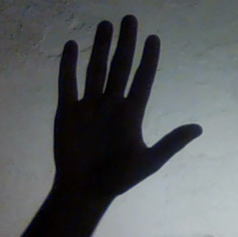
\includegraphics[width=\linewidth]{Hand-Original.png}
    \caption*{(a) Original Image}
  \end{minipage}
  \hfill
  \begin{minipage}[b]{0.48\linewidth}
    \centering
    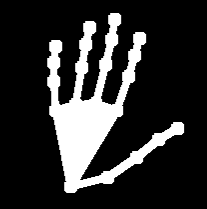
\includegraphics[width=\linewidth]{Hand-Result.png}
    \caption*{(b) Segmented Result}
  \end{minipage}
  \caption{Example of the segmentation process: (a) the original hand image; (b) the resulting binary mask after segmentation using our Mediapipe-based algorithm.}
  \label{fig:segmentation}
\end{figure}




\section{Experiments}
Our experiments helped to define the optimal parameters for the SVM and our measured features for our gesture recognition
problem. These experiments were held as A - B style tests where two methods with one differing parameter were compared. The results of these tests are shown in 

\begin{figure}[htb]
  \centering
  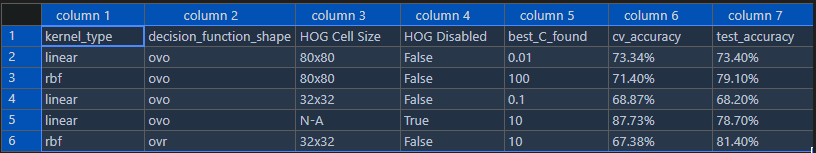
\includegraphics[width=\linewidth]{Testing-Results.png}
  \caption*{Pre-final model AB testing results.}
\end{figure}

\noindent\textbf{Results Summary} These AB tests helped us conclude many parameters for our final model. First of which was
a linear vs non-linear kernel. Using linear and rbf kernels on otherwise identical models showed us that
the rbf kernel lowered our cross-validation accuracy and increased our test accuracy. This widening of the gap between
the validation and test accuracy shows inconsistency for the rbf-using model. This inconsistency was likely a sign of the non-linear
kernel picking up some patterns more strongly causing it to underperform on average across CV folds.
A HOG descriptor cell size of 80x80 was also tested against a 32x32 cell size. The 80x80 cell size was able to achieve a higher
cross-validation accuracy of 73.34\% vs 68.87\% for the 32x32 cell size. The test accuracy was also higher at 73.40\% vs 68.20\%.
The larger size (less descriptors) achieving a higher accuracy was very surprising as the 80x80 model had a lot less to work with.
I think this may be explained however by the fact that more HOG descriptors likely meant less valuation of the 7 Hu moment descriptors.
This analysis is supported by the fact that the HOG descriptor disabled model managed to outperform all of the other models with HOG descriptors enabled
during these tests with a staggering 87.73\% CV accuracy and a less impressive test accuracy of 78.70\%.
One-vs-Rest was also tested in a not exactly AB style but its CV performance was hurt by about 4 percentage points
despite the fact that it had more than double the HOG descriptors which hurt the a previous AB test with run 1 and 3 by about 5 percentage points.
It's therefore likely running OvR only increased the performance by about 1 percentage point which can be considered negligible. This analysis however is
not considering the fact that the OvO vs. OvR runs were both non-linear while the 80x80 vs. 32x32 runs were both linear. This is another
variable that can likely skew this analysis either way and more tests would be needed to determine the true impact of the OvO vs. OvR.

\noindent\textbf{Other Parameters Experimentally Set} Please note that for each of model trained, the Hyperparameter C is selected via
leave-one-subject-out (LOSO) cross-validation. C was selected from the set of \{0.01, 0.1, 1, 10, 100\} and the best performing C was used for each model.


\section{Results and Discussion} 

The final model was trained with the parameters and features described in Table 1.

\begin{table}[h]
\centering
\scriptsize
\begin{tabular}{l l l c c c c}
\hline
Kernel & Decision & HOG Cell & HOG & C & CV Acc. & Test Acc. \\
Type   & Shape    & Size     & Disabled &  &  &  \\
\hline
linear & ovo & 80×80 & False & 0.001 & 85.96\% & 90.58\% \\
\hline
\end{tabular}
\caption{Final SVM configuration and performance.}
\end{table}

\medskip
\noindent\textbf{Quantitative Results}

\begin{figure}
  \centering
  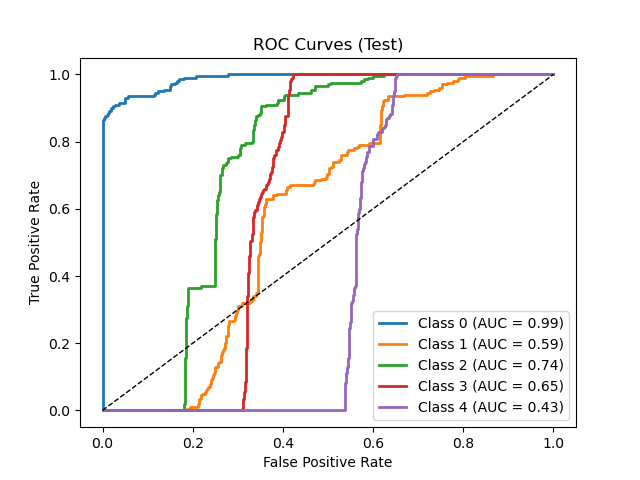
\includegraphics[width=\linewidth]{ROC_Test.png}
  \caption*{ROC test results (each gesture’s true‑positive rate (TPR) versus false‑positive rate (FPR)).}
\end{figure}

\begin{figure}
  \centering
  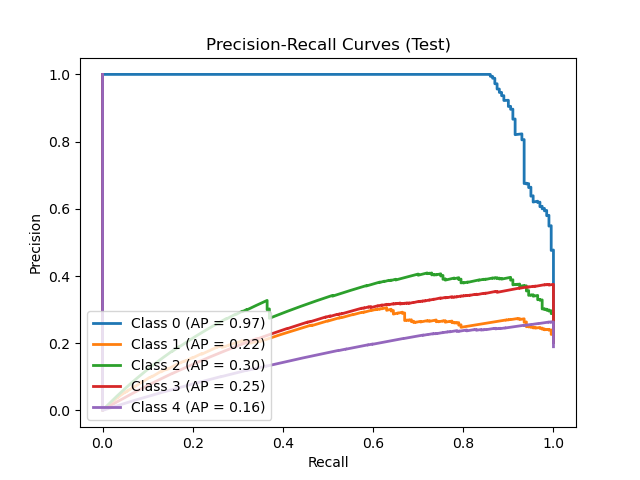
\includegraphics[width=\linewidth]{PR_Test.png}
  \caption*{PR test results. Shows we're most precise with the Palm gesture, this makes sense as virtually no palm gestures were removed due to segmentation error and its also the most basic of gestures. The late decline of the other gesture classes suggests that as soon as we try to capture a substantial fraction of those gestures, we incur a huge number of false positives.}
\end{figure}

\begin{figure}
  \centering
  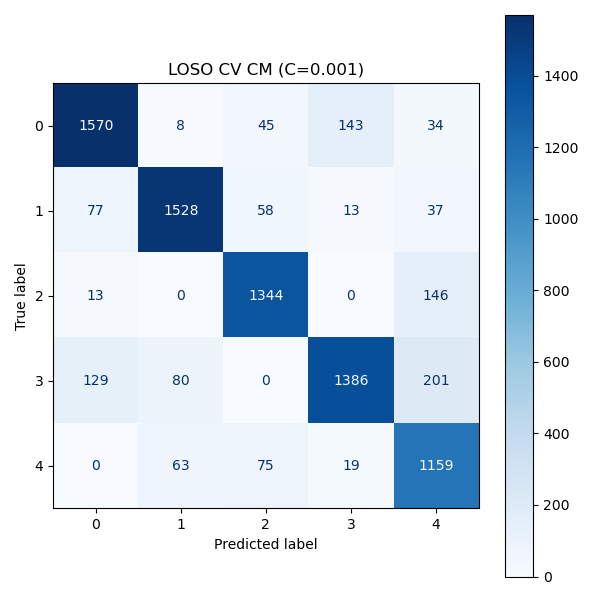
\includegraphics[width=\linewidth]{CM-linear-ovo-80x80-True-False-CV_new-new.png}
  \caption*{Validation confusion matrix. Shows most mistakes are between OK and C gestures, with a decent amount of OK and Palm confusion as well.} 
\end{figure}

\begin{figure}
  \centering
  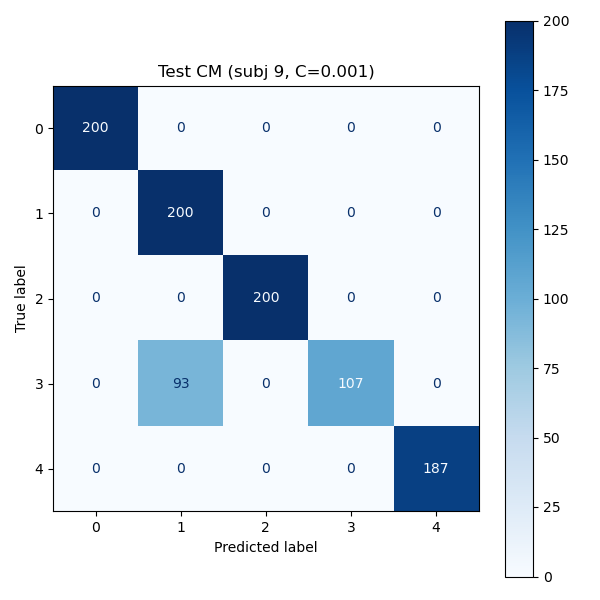
\includegraphics[width=\linewidth]{CM-linear-ovo-80x80-True-False-Test_new_new.png}
  \caption*{Test confusion matrix.}
\end{figure}

\begin{table}
  \centering
  \scriptsize
  \begin{tabular}{l c c c c}
  \hline
  \textbf{Label} & \textbf{Precision} & \textbf{Recall} & \textbf{F1‑score} & \textbf{Support} \\
  \hline
  0           & 0.88 & 0.87 & 0.87 & 1800 \\
  1           & 0.91 & 0.89 & 0.90 & 1713 \\
  2           & 0.88 & 0.89 & 0.89 & 1503 \\
  3           & 0.89 & 0.77 & 0.83 & 1796 \\
  4           & 0.73 & 0.88 & 0.80 & 1316 \\
  \hline
  \textbf{Accuracy}    & \multicolumn{3}{c}{0.86} & 8128 \\
  \textbf{Macro avg}   & 0.86 & 0.86 & 0.86 & 8128 \\
  \textbf{Weighted avg}& 0.86 & 0.86 & 0.86 & 8128 \\
  \hline
  \end{tabular}
  \caption{Classification report on cross‑validation (LOSO) set.}
\end{table}
  
\begin{table}
  \centering
  \scriptsize
  \begin{tabular}{l c c c c}
  \hline
  \textbf{Label} & \textbf{Precision} & \textbf{Recall} & \textbf{F1‑score} & \textbf{Support} \\
  \hline
  0           & 1.00 & 1.00 & 1.00 & 200 \\
  1           & 0.68 & 1.00 & 0.81 & 200 \\
  2           & 1.00 & 1.00 & 1.00 & 200 \\
  3           & 1.00 & 0.54 & 0.70 & 200 \\
  4           & 1.00 & 1.00 & 1.00 & 187 \\
  \hline
  \textbf{Accuracy}    & \multicolumn{3}{c}{0.91} & 987 \\
  \textbf{Macro avg}   & 0.94 & 0.91 & 0.90 & 987 \\
  \textbf{Weighted avg}& 0.94 & 0.91 & 0.90 & 987 \\
  \hline
  \end{tabular}
  \caption{Classification report on held‑out test subject (Test accuracy: 90.58\%).}
\end{table}

\medskip
\noindent\textbf{Qualitative and Quantitative Result Analysis}
From testing on the video stream running the final model, I observed that the model 
had a really hard time specifically recognizing the OK and C gestures. This is likely for a few reasons.
Firstly, both gestures have very similar rounded shapes with two connecting fingers. This specific confusion
is backed clearly by the entries in the confusion matrix and in figures 9 and 10. Secondly,
these two gestures were by far the most thrown out during the segmentation of the data. Meaning,
that mediapipe failed to find a hand most often with these gestures. This imbalance likely caused the
model to simply be more right more often just going safely with another more common gesture.
In retrospect, this imbalance could have been easily avoided by supplementing the data, or 
removing some gestures from the more common classes.
In addition to this, it seems that the live camera version also just struggles in general,
not just with the OK and C gestures. We think this could be caused by a few key differences between my video stream and the dataset. These differences include
hand orientation, distance from the camera and a lack of warping due to high-fov camera used in the dataset.
All of these factors can help explain why the model is specifically poorer when working with my live feed compared to other subjects in the same dataset where it had ~90\% test accuracy and ~86\% validation accuracy.




\begin{figure}
  \centering
  
\includegraphics[width=\linewidth]{input1.png}
  \caption*{OK gesture recognized as C gesture. This mistake
  is understandable as both gestures have similar hand shapes and this
  particular example could be questionable even to a human as to whether it is a C or an OK.
  This may be a result of bad data: either the image was too poor / stretched for the mediapipe
  hands to get a good read, or the original gesture itself was ambiguous.}
\end{figure}

\begin{figure}
  \centering
  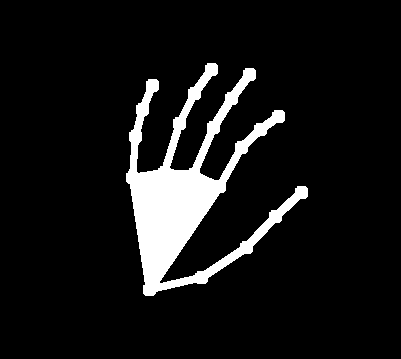
\includegraphics[width=\linewidth]{input2.png}
  \caption*{Palm gesture recognized as OK gesture. This mistake is decipherable as
  this particular example does have a rounded right side which could be confused for the round
  right side shaping of the OK gesture.}
\end{figure}

\begin{figure}
  \centering
  
\includegraphics[width=\linewidth]{input3.png}
  \caption*{Thumb gesture recognized as Palm gesture. This
  mistake is a clear result of a failure of the mediapipe hand mask segmentation as the hand
  looks jumbled as is unrecognizable as any of the 5 classes of gestures measured.}
\end{figure}
  


\nocite{Aurangzeb2023, Mahmood2024, Miron2019, Panduranga2018, Premaratne2014, Dalal2005}

% \section{Timeline}
% \textbf{March 3 -- April 25, 2025}: 
% \begin{itemize}
%     \item \textbf{March 3--9:} Project setup, literature review, and environment configuration.
%     \item \textbf{March 10--16:} Data collection and preparation, including processing the Leap Motion dataset.
%     \item \textbf{March 17--23:} Development and refinement of the Mediapipe-based hand segmentation algorithm.
%     \item \textbf{March 24--30:} Implementation of feature extraction methods (HOG, Hu moments).
%     \item \textbf{March 31--April 6:} Non-linear SVM classification implementation and hyperparameter tuning.
%     \item \textbf{April 7--April 13:} System integration and initial real-time testing.
%     \item \textbf{April 14--April 20:} Optimization of the processing pipeline, including experiments to reduce the number of features and utilize a lower-dimensional HOG representation, as well as extensive robustness testing.
%     \item \textbf{April 21--April 25:} Final system refinement, documentation, and report preparation.
% \end{itemize}

\section{Future Work}
To better our solution to the problem of gesture recognition, the
first step is clear; ascertaining a better dataset. This is most
obviously highlighted by the relative success of the model amongst the dataset with
validation and test accuracies mentioned, but the failure of the model to generalize to our own webcam feed.
As a next step, we would like to use my get-more-data.py script to collect a large dataset of my own, taking into
account some of the potential issues with the leap Gesture dataset and my approach such as orientation of the hand,
hand distance from the camera as well as general compliance with the mediapipe hand segmentator (so better lighting more 
common camera settings). Furthermore, exploring this problem with a deep learning approach could be a good next step.
First, we could fine‑tune a lightweight convolutional neural network—such as MobileNetV2 or EfficientNet‑Lite—directly on our 640×480 binary hand masks, allowing the network to learn feature hierarchies optimized for gesture contours rather than relying solely on hand‑crafted HOG and Hu descriptors. Second, we can build a hybrid model that concatenates the pre‑trained CNN’s penultimate embedding with our HOG+Hu feature vector, then feeds the combined representation into a fully connected classification head; this “late fusion” approach has been shown to leverage both learned texture‐invariant features and explicit shape descriptors. Training such a fusion network end‑to‑end (or in two stages) would enable the classifier to weight CNN features against HOG/Hu inputs dynamically, potentially boosting accuracy, improving robustness to segmentation noise, and reducing our dependence on manual feature engineering.
Some obvious drawbacks of switching to this kind of architecture however revolves around the need for an even bigger dataset - which is currently the likely source of our existing troubles.


\section{References}
\bibliographystyle{IEEEbib}
\bibliography{refs}

\end{document}


